\documentclass[11pt]{exam}
\usepackage[margin=1in]{geometry}
\pagestyle{plain}
\usepackage{amsmath,amsfonts,amssymb,amsthm,enumerate}
\usepackage{multicol}
\usepackage[]{graphicx}
\usepackage{hyperref}
\usepackage{tikz}
\usepackage{pgfplots}
\usepackage{subfigure}
\usepackage[final]{pdfpages}

\addtolength{\footskip}{2\baselineskip} % to lower the page numbers
\title{\vspace{-0.5in} Math 115 \\ Worksheet Section 4.6}
\date{}


% \theoremstyle{definition}
% \newtheorem{problem}{Problem}
\renewcommand{\questionlabel}{\textbf{Problem~\thequestion.}}
%\printanswers

\begin{document}
\maketitle
\vspace{-0.75in}
\section*{Steps for related rates problems}
\begin{enumerate}
\item Draw a picture and define important variables.
\item Identify the
  quantity for which we want to compute the rate of change. Find a
  formula for it.
\item Treat each quantity in your equation as a
  function of time, and then take the derivative of both sides with
  respect to time.
\item Substitute any given quantities and rates of
  change into your derivative equation, paying particularly close
  attention to the sign of any rates of change.
\item If any quantity or
  rate of change (other than the one we want to compute) in your
  derivative equation is still unknown, see if you can use the
  original equation or any other equations relating the quantities to
  solve for those unknowns.
\item Use your derivative equation to solve
  for the desired rate of change.
\end{enumerate}
\begin{questions}
  \question A plane is climbing at \(500\) feet per minute, and the
    air temperature outside the plane is falling at \(2^\circ\)C per
    \(1000\) feet. What is the rate of change (as a function of time)
    of the air temperature just outside the plane?
    \begin{solution}
      \begin{enumerate}
      \item Let \(y\) be the height of the airplane and \(T\)
        be the air temperature.
      \item We wish to compute \(\frac{dT}{dt}\). We know \(T =
        T_0-\frac{2}{1000}y\) for \(T_0\) the temperature at height
        \(0\) feet.\\
      \item Taking the derivative of our equation above, we get \[
          \frac{dT}{dt} = -\frac{2}{1000} \frac{dy}{dt}
        \]
      \item We know that \(\frac{dy}{dt} = 500\) feet/minute from the
        problem. Thus, \[
          \frac{dT}{dt} = -\frac{2}{1000}(500) = -1^\circ \text{C per minute}
        \]
      \end{enumerate}
    \end{solution}
  \question The gravitational force, \(F\), on a rocket at a distance,
    \(r\), from the center of the earth is given by \[
      F = \frac{k}{r^2}
    \]
    where \(k = 10^{13}\) newton \(\cdot\) km\({}^2\). When the rocket
    is \(10^4\) km from the center of the earth, it is moving away at
    \(0.2\) km/sec. How fast is the gravitational force changing at
    that moment? Give units. (A newton is a unit of force.)
    \begin{solution}
      \begin{enumerate}
      \item We already have all our variables defined.
      \item We wish to compute \(\frac{dF}{dt}\). We already have an
        equation for \(F\) given.
      \item Taking its derivative, we get \[
          \frac{dF}{dt} = -2 \frac{k}{r^3} \frac{dr}{dt}
        \]
      \item We know that \(\frac{dr}{dt} = 0.2\) km/sec and \(r =
        10^4\). Thus, \[
          \frac{dF}{dt} = -2 \frac{10^{13}}{(10^4)^3} (0.2) = -4 \text{newton/sec}
        \]
      \end{enumerate}
    \end{solution}
  \question The average cost per item, \(C\), in dollars, of
    manufacturing a quantity \(q\) of cell phones is given by \[
      C = \frac{a}{q}  + b, \quad \text{where }a,b\text{ are positive constants.}
    \]
    \begin{enumerate}[(a)]
    \item Find the rate of change of \(C\) as \(q\) increases. What
      are its units?
    \item If production increases at a rate of \(100\) cell phones per
      week, how fast is the average cost changing? Is the average cost
      increasing or decreasing?
    \end{enumerate}
    \begin{solution}
      \begin{enumerate}[(a)]
      \item \[
          \frac{dC}{dq} = -\frac{a}{q^2} \text{ dollars/cell phone}
        \]
      \item We wish to find \(\frac{dC}{dt}\) given that
        \(\frac{dq}{dt} = 100\). We solve \[
          \frac{dC}{dt} = -\frac{a}{q^2} \frac{dq}{dt} =
          -\frac{a}{q^2}100
        \]
        so average cost is decreasing since \(a\) is positive.
      \end{enumerate}
    \end{solution}
  \question Car B is driving south, away from an intersection.  Car A is approaching the intersection and is moving west.  At what rate is the distance between the cars changing at the instant when car B is 40 miles from the intersection and traveling 50 mph and car A is 30 miles from the intersection and traveling at 45 mph?  Are the cars getting closer together or farther apart at this time?
    \begin{solution}
      Let \(y\) be the distance from Car B from the intersection. Let
      \(x\) be the distance of Car A from the intersection. Let \(z\)
      be the distance between the two cars.
      \begin{center}
        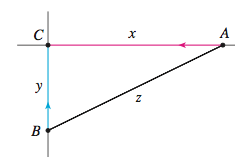
\includegraphics[scale=0.7]{cars-at-intersection}
      \end{center}
      \textbf{Method 1:} Then, we know \[
        z^2 = x^2 + y^2
      \]
      and thus \[
        2z\frac{dz}{dt}  = 2x\frac{dx}{dt} + 2y\frac{dy}{dt}
      \]
      Substituting \(\frac{dx}{dt} = -45, x=30, \frac{dy}{dt} = 50,
      y=40\), and \(z = \sqrt{30^2+40^2} = 50\), we get \[
        2(50) \frac{dz}{dt} = 2(30)(-45) + 2(40)(50)
        \implies\frac{dz}{dt}  = \frac{-1350+2000}{50} =
        \frac{650}{50} = 13 \text{ miles per hour}
      \]
      \textbf{Method 2:} Then, we know \[
        z = \sqrt{x^2+y^2}
      \]
      and thus \[
        \frac{dz}{dt} = \frac{1}{2} (x^2+y^2)^{-1/2}\left(2x\frac{dx}{dt}+2y\frac{dy}{dt}\right)
      \]
      Substituting \(\frac{dx}{dt} = -45, x=30, \frac{dy}{dt} = 50,
      y=40\), we get \[
        \frac{dz}{dt} = \frac{1}{2}
        (30^2+40^2)^{-1/2}\left(2(-45)(30)+2(40)(50)\right)
        =\frac{1}{2}\cdot \frac{1}{50}(-2700+4000) = \frac{1300}{100}
       = 13\text{ mph}
      \]
      In both methods, we see the cars are getting farther apart.
    \end{solution}
\question (Winter 2017 Final Exam) % problem 5
A cylindrical bar of radius $R$ and length $L$ (both in meters) is put into an oven. As the bar gains temperature, its radius decreases at a constant rate of 0.05 meters per hour and its length increases at a constant rate of 0.12 meters per hour. Fifteen minutes after the bar was put into the oven, its radius and length are 0.4 and 3 meters respectively. At what rate is the volume of the bar changing at that point? Be sure to include units.
\begin{solution}
  See \href{https://dhsp.math.lsa.umich.edu/exams/115exam3/w17/s5.pdf}{https://dhsp.math.lsa.umich.edu/exams/115exam3/w17/s5.pdf}
\end{solution}
\question (Winter 2016 Final Exam) % problem 3
A man, who is 28 feet away from a 30 foot tall street lamp, is sinking into quicksand. (See diagram below.) At the moment when 6 feet of him are above the ground, his height above the ground is shrinking at a rate of 2 feet/second.
\begin{center}
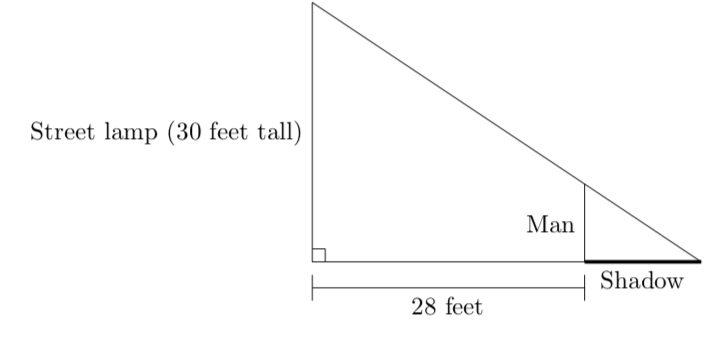
\includegraphics[scale=0.5]{shadow.png}
\end{center}
\begin{enumerate}[(a)]
\item How long will the man's shadow (shown in bold in the diagram above) be at the moment when 6 feet of him are above the ground?
\item At what rate is the length of the man's shadow changing at the moment 6 feet of him are above the ground? Is his shadow growing or shrinking at that moment?
\end{enumerate}
\begin{solution}
  See \href{https://dhsp.math.lsa.umich.edu/exams/115exam3/w16/s3.pdf}{https://dhsp.math.lsa.umich.edu/exams/115exam3/w16/s3.pdf}
\end{solution}
\question (Fall 2014 Final Exam) % problem 5
Tommy and Gina were friends in high school but then went to college in different parts of the country. They thought they were going to see each other in Springfield over the December break, but their schedules didn't match up. In fact, it turns out that Tommy is leaving on the same day that Gina is arriving.
Shortly before Gina's train arrives in Springfield, she sends a text to Tommy to see where he is, and Tommy sends a text response to say that, sadly, his train has already left. At the moment Tommy sends his text, he is 20 miles due east of the center of the train station and moving east at 30 mph while Gina is 10 miles due south of the train station and moving north at 50 mph.
\begin{enumerate}[(a)]
\item What is the distance between Gina and Tommy at the time Tommy sends his text? Remember to include units.
\item When Tommy sends his text, are he and Gina moving closer together or farther apart? How quickly? You must show your work clearly to earn any credit. Remember to include units.
\item Let $J(t)$ be the distance between Gina and Tommy t hours after Tommy sends his text. Use the local linearization of $J(t)$ at $t = 0$ to estimate the distance between Gina and Tommy 0.1 hours after Tommy sends his text. Remember to show your work carefully.
\end{enumerate}
\begin{solution}
  See \href{https://dhsp.math.lsa.umich.edu/exams/115exam3/f14/s5.pdf}{https://dhsp.math.lsa.umich.edu/exams/115exam3/f14/s5.pdf}
\end{solution}
\end{questions}
\end{document}
%%% Local Variables:
%%% mode: latex
%%% TeX-master: t
%%% End:
